\chapter{Conclusions} \label{ch:conclusion}

% Main points:
% - What has been accomplished that was not there before
% - What is the most relevant follow up work
% - What are the most relevant challenges
% - Make sure to connect with the introduction, that is refer to the problems presented there and the degree to wich they are addressed.

% Paragraph structure
% 1. Accomplishments
% 2. Next wave: The need of the problem framing to build and study strains in this context
% 3. Future persepective (be general and tie back to the intro, but still make this "contribute my grain of sand)


\begin{figure}[h]
  \centering
  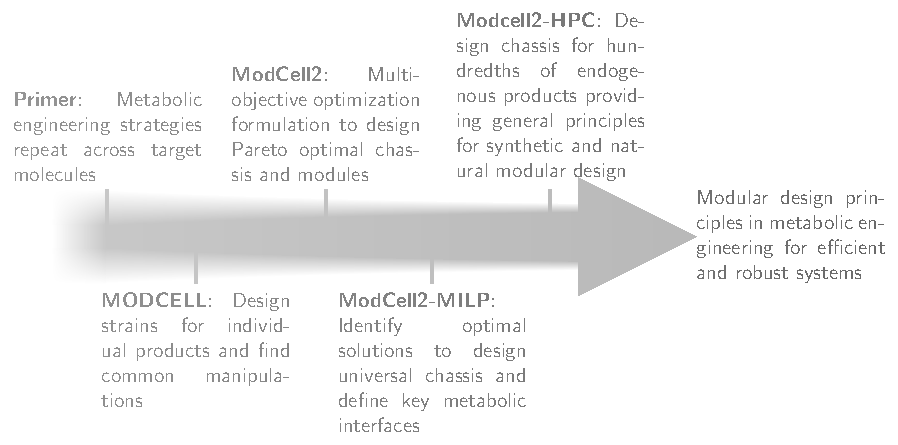
\includegraphics[width=\textwidth]{timeline-arrow}
    \caption{Advances of this thesis}
\end{figure}
